%-------------------------------------------------------------------------------
\subsubsection{Exemple de fonction de $\Rbb^2 \mapsto \Rbb$}
%-------------------------------------------------------------------------------

Soit la fonction $f: \Rbb^2 \mapsto \Rbb$ définie par
$$
f(x, y) = x^3 + y^3 - 3 xy
$$

\begin{enumerate}
  \item Déterminer les points stationnaires de la fonction $f$.
  \solution{
    Le gradient de $f$ vaut
    $$
    \nabla f = \left[\begin{array}{c} 3x^2 - 3y \\ 3y^2 - 3x \end{array}\right]
    $$
    qui est nul aux points
    $$
    a = (0, 0) \qquad \text{et} \qquad b = (1, 1).
    $$
  }
  \item Déterminer s'il s'agit de maximums, de minimums ou de points selles.
  \solution{
    La hessienne vaut
    $$
    \nabla^2 f = \left[\begin{array}{rrr} 6x & & -3 \\ -3 & & 6y \end{array}\right].
    $$
    \begin{description}
      \item[\'Etude du point $a$ :] on a 
      $$
      \nabla_a^2 f = \left[\begin{array}{rrr} 0 & & -3 \\ -3 & & 0 \end{array}\right]
      \qquad \Rightarrow \qquad 
      | \nabla_a^2 f | = -9 < 0
      $$
      donc $a$ est un point selle. Ses valeurs propres sont les racines de
      $$
      P(\lambda) = \left|\begin{array}{rrr} -\lambda & & -3 \\ -3 & & -\lambda \end{array}\right|
      = \lambda^2 - 9 
      \qquad \text{soit} \quad 
      \lambda = \pm 3.
      $$
      Tout vecteur propre associé à $\lambda = -3$ est solution de 
      $$
      \left\{\begin{array}{rcl} -3y & = & -3x \\-3x & = & -3y\end{array} \right.
      \qquad \Rightarrow \qquad 
      x = y
      \qquad \Rightarrow \qquad 
      \left[ \begin{array}{r} 1 \\ 1 \end{array} \right] \text{ est associé à $-3$}
      $$
      donc $a$ est un maximum dans la direction de la 1ère bissectrice. \\
      Tout vecteur propre associé à $\lambda = 3$ est solution de 
      $$
      \left\{\begin{array}{rcl} -3y & = & 3x \\-3x & = & 3y\end{array} \right.
      \qquad \Rightarrow \qquad 
      x = -y
      \qquad \Rightarrow \qquad 
      \left[ \begin{array}{r} -1 \\ 1 \end{array} \right] \text{ est associé à $+3$}
      $$
      donc $a$ est un minimum dans la direction de la 2ème bissectrice.
      $$
      \begin{tabular}{cc}
        direction $x = y$ & direction $x = -y$ \\
        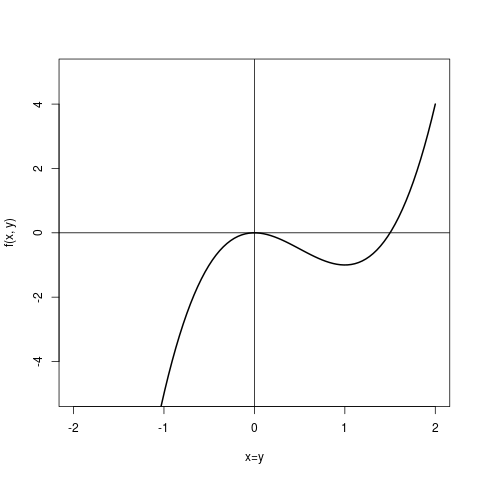
\includegraphics[width=.35\textwidth, trim=00 10 10 40, clip=]{ExempleOptimum-1ereBissectrice} &
        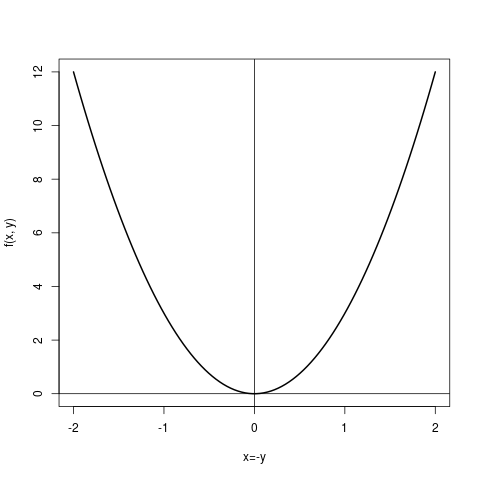
\includegraphics[width=.35\textwidth, trim=00 10 10 40, clip=]{ExempleOptimum-2emeBissectrice} \\
        $f(x, x) = 2x^3 - 3x^2$ & $f(x, -x) = 3x^2$
      \end{tabular}
      $$
      \item[\'Etude du point $b$ :] on a
      $$
      \nabla_b^2 f = \left[\begin{array}{rrr} 6 & & -3 \\ -3 & & 6 \end{array}\right]
      \qquad \Rightarrow \qquad 
      | \nabla_b^2 f | = 27 > 0, \qquad \tr(\nabla_b^2 f) = 12 > 0
      $$
      donc les deux valeurs propres de $\nabla_b^2 f$ sont positives : $b$ est donc un minimum.
    \end{description}
    Au total la surface d'équation $\{z = f(x, y)\}$ a l'aspect suivant
    $$
    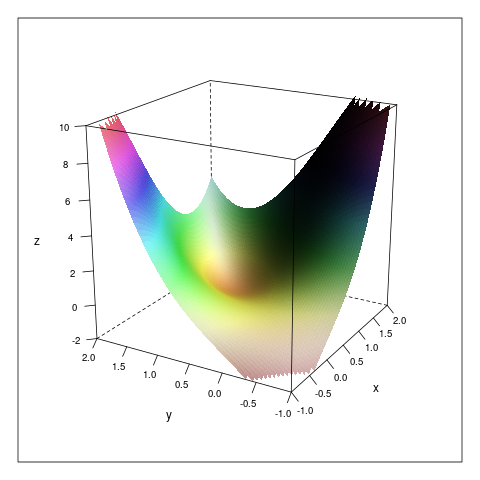
\includegraphics[width=.6\textwidth]{ExempleOptimum-surface}
    $$
  }
\end{enumerate}
